\documentclass[11pt]{article}
\usepackage{common/acl-ijcnlp2009}
\usepackage{times}
\usepackage{latexsym}
\usepackage{common/prettyref}
\usepackage{common/jeffe}
\usepackage{common/hyphen}
\usepackage{latexsym}
\usepackage{subfigure}
\usepackage{graphicx}
\usepackage[applemac]{inputenc}

\newrefformat{tab}{Table \ref{#1}} 
\newrefformat{fig}{Figure \ref{#1}} 
\newrefformat{eqn}{(\ref{#1})} 
\newcommand{\ignore}[1]{}


\newcommand{\nt}[2]{\textrm{#1}_{\framebox[5pt]{\scriptsize #2}}}
\newcommand\bleu{\textsc{Bleu}}
\newcommand\giza{{GIZA++}}
\newcommand\boe{\mathbf{e}}
\newcommand\bof{\mathbf{f}}
\newcommand{\ind}[1]{{\fboxsep1pt\raisebox{-.5ex}{\fbox{{\tiny #1}}}}}
% allows margin notes
%\newcommand\margin[1]{} % hide them!!!
\newcommand\margin[1]{\mbox{}\marginpar{\raggedright\hspace{0pt}\tiny\em#1}}
\addtolength{\marginparwidth}{-3ex}

\newcommand{\ts}{\ensuremath{\vec{t}}}
\newcommand{\es}{\ensuremath{\vec{e}}}
\newcommand{\rs}{\ensuremath{\vec{r}}}
\newcommand{\condon}{\hspace{0pt} | \hspace{1pt}}
\newcommand{\but}[2]{\ensuremath{{\bf #1}_{-#2}}}
\newcommand{\blt}[2]{\ensuremath{{\bf #1}_{<#2}}}
\newcommand{\pu}{\ensuremath{P_0}}
\renewcommand{\vec}[1]{{\bf #1}}
\newcommand{\emin}{\ensuremath{\es^-}}

\newcommand{\bibsnip}{\vspace{-1ex}}

%% sloppy linebreaks
%\sloppy

%% no extra spacing after dots
%\frenchspacing

\makeatletter
\setlength{\columnsep}{3mm} % this one's nasty!!!

%\setlength{\topmargin}{0in}
%\setlength{\headheight}{0in}
%\setlength{\headsep}{-0.2in}
\setlength{\textheight}{10.0in}
%\setlength{\oddsidemargin}{0in}
%\setlength{\textwidth}{6.5in}
\setlength\titlebox{1.0in}
\renewcommand{\baselinestretch}{0.965}
\setlength{\textfloatsep}{3mm}
\setlength{\floatsep}{1.5mm}


\title{Models of Synchronous Grammar Induction for SMT}
\author{
  Phil Blunsom\\ 
  %\vspace{6pt} 
  Phil.Blunsom@comlab.ox.ac.uk\\
%  {\rm $^*$Computing Laboratory}\\
  University of Oxford\\
% \And
%  Alex Clark\\
%  %\vspace{6pt} 
%  alexc@cs.rhul.ac.uk\\
%%  {\rm $^\textrm{\textdagger}$Department of Computer Science}\\
%  Royal Holloway University
% \And
%  Trevor Cohn\\
%  %\vspace{6pt} 
%  T.Cohn@dcs.shef.ac.uk\\
%%  {\rm $^\textrm{\textdagger}$Department of Computer Science}\\
%  University of Shefield
%\\
% \AND
%  Chris Dyer\\
%  %\vspace{6pt} 
%  redpony@umd.edu\\
%%  {\rm $^\textrm{\textdagger}$Department of Computer Science}\\
%  University of Maryland
% \And
%  Adam Lopez\\
%  %\vspace{6pt} 
%  alopez@inf.ed.ac.uk\\
%%  {\rm $^\textrm{\textdagger}$Department of Computer Science}\\
%  University of Edinburgh 
}

\begin{document}
\maketitle

%\begin{abstract}
%Synchronous grammar transducers have made a big impact in the field of machine translation in recent years. 
%However, current techniques for acquiring translation grammars are either overly simplistic or else too heavily reliant on the availability of high-quality statistical parsers.
%We propose the development of algorithms for large-scale unsupervised synchronous grammar induction. 
%Using advanced clustering techniques from machine learning we aim to induce grammars which use a rich set of non-terminals, %, in contrast to many existing approaches which have only one.
%thereby producing high quality translation models for language pairs solely using a parallel corpus. %, without relying on treebank parsers.
%\end{abstract}

%%Research into statistical machine translation has changed dramatically in recent years with the introduction of grammar-based transducers (e.g., Chang's Hiero and USC/ISI's syntax-based system). 
%A critical component of synchronous grammar translation models is their \emph{grammar} which encodes translational equivalence and licenses reordering between tokens in the source and target languages. 
%There is considerable scope for improving beyond current techniques for automatically acquiring synchronous grammars from bilingual corpora, which seek to find either extremely simple grammars with only one non-terminal or else rely on treebank-trained parsers.
%The simple grammars are incapable of representing constituency information, while the richer grammars limit the systems' portability to new target languages while enforcing a restrictive notion of linguistic constituency. 
%Instead we propose to develop an unsupervised method for large-scale unsupervised synchronous grammar induction using multiple non-terminal symbols to represent contextual information.
%In such a way we can harness the benefits of a richer grammar without the limiting data requirements or linguistic constraints.

The last decade of research in Statistical Machine Translation (SMT) has seen rapid progress. %with small scale research systems maturing into large commercial products and ubiquitous online tools. %\footnote{e.g., translate.google.com, www.systran.co.uk, www.languageweaver.com} 
Unfortunately these successes have not been uniform; 
%current state-of-the-art translation output varies markedly in quality depending on the languages being translated. 
%Those language pairs that are 
closely related language pairs 
%(e.g., English and French) 
can be translated with a high degree of precision, while for distant pairs 
%(e.g., English and Chinese) 
the result is far from acceptable. 
%It is tempting to argue that SMT's current limitations can be overcome simply by increasing the amount of data on which the systems are trained. 
%However, large scale evaluation campaigns for Chinese~$\rightarrow$~English translation have not yielded the expected gains despite the increasing size of the models. 
%While many researchers are tackling these issues, their proposed solutions are limited by focusing on more expressive models of translation rather than addressing the issue of how, and what, translation units are learnt a priori.

Models which have been most successful for translating between structurally divergent language pairs have been based on synchronous grammars. 
%However these successes have been tempered by a reliance on high quality monolingual parse trees on the output side of the translation model, severely restricting the applicability of such models to the case of translating into English.
A critical component of these translation models is their \emph{grammar} which encodes translational equivalence and licenses reordering between tokens in the source and target languages. 
There is considerable scope for improving beyond current techniques for automatically acquiring synchronous grammars from bilingual corpora, which seek to find either extremely simple grammars with only one non-terminal or else rely on treebank-trained parsers.
The simple grammars are incapable of representing the substitutability of a constituent, while the richer grammars limit the systems' portability to new target languages (effectively limiting us to translating into/out of English) while enforcing a restrictive notion of linguistic constituency (Figure \ref{fig:models}). 
%A further, but more subtle, limitation of these models is the assumption that the particular brand of linguistic structure assigned by a parser (usually a form of phrase structure grammar learnt from the Penn. Treebank) is predominantly isomorphic to that of the input language; an assumption which is rarely true for distantly related language pairs (or even closely related ones: Figure \ref{fig:models}).

Clearly there is a need for research into the unsupervised induction of synchronous grammar based translation models.
%Previous research has focussed on structured learning approaches requiring costly global inference over translation pair derivations, limiting the ability of these models to be scaled to large datasets.
We propose the pragmatic approach of embracing existing algorithms for inducing unlabelled SCFGs (e.g. the popular Hiero model), and then using state-of-the-art hierarchical non-parametric Bayesian models to independently learn syntactic classes for translation rules in the grammar.


The agenda of the workshop will address two goals: (1) to implement and systematically investigate the performance of current synchronous grammar based SMT systems, focusing on the role of constituency and syntactic classes in informing translation structure; (2) to develop scalable unsupervised algorithms for assigning labels to translation rules in synchronous grammars. 
These algorithms will be implemented within the {\em Joshua} decoder with the intention of providing an open source implementation of the existing and proposed synchronous grammar SMT systems.

\paragraph{1) Systematic comparison of synchronous grammar based SMT} 
Firstly we will extend the Joshua decoder to handle a range of the currently proposed synchronous grammar based SMT models.
Through experimentation on a range of parallel corpora (small and large, hi and low density languages), we will systematically explore the question of what the most effective models of synchronous syntax for SMT are.
%Previous work has assumed a linguistic motivation, but there is a compelling argument that a more appropriate representation may be one which specifically addresses the divergence between a given language pair (Figure~\ref{fig:models}).
%Such a grammar might simply encode the number of tokens in the constituent being generated, the number of reordering operations on the path from the root to that constituent, or whether a constituent prefers to reorder in a specific direction.

\paragraph{2) Unsupervised learning of labelled synchronous grammars} 
The second goal will be to apply unsupervised Bayesian techniques, such as Latent Dirichlet Allocation (LDA) and hierarchical non-parametric models (HDPs, HPYPs), to the task of assigning equivalence classes to phrase translations.
Inspired by work in monolingual PCFG learning, we will investigate generative models which describe the production of phrase translations in terms of sequences of tokens (or word classes) and their observed contexts.

We have put together an enviable superset of faculty and graduate students from which the senior members of the workshop will be drawn: Joy Ying Zhang (CMU), Trevor Cohn (Sheffield), Alex Clark (RHUL), Chris Dyer (UMD), Adam Lopez (Edinburgh), Yang Liu (CAS), Zhifei Li (JHU) and Andreas Zollmann (CMU). 

The success of the workshop will impact widely on both the machine translation community, and the field of grammar induction.
By investigating our stated goals in the context of a CLSP workshop we will provide a deep understanding of synchronous grammar based SMT; both generating interest and furthering research into widely applicable unsupervised techniques for synchronous grammar induction. 
Such techniques promise to bring high performance SMT models, only currently applicable to working with English, to the full range of languages of the world.
In addition we will provide a benchmark implementation of synchronous grammar based SMT models ready for wide adoption within the SMT research community.

\begin{figure}
% \subfigure[Formal syntax]{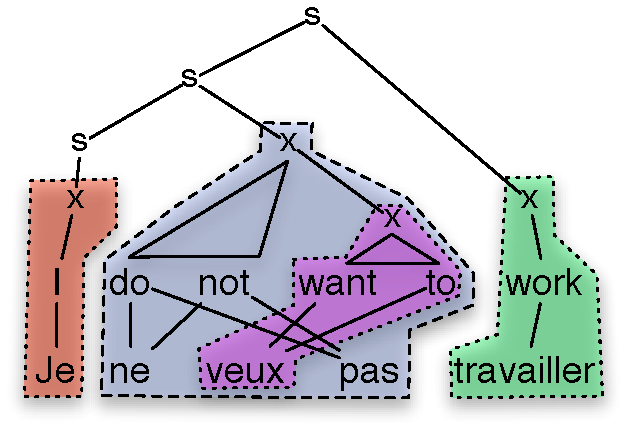
\includegraphics[scale=0.2]{JeNeVeuxPasTravailler-Hiero.pdf}}
  \subfigure[Unsupervised syntax]{\includegraphics[scale=0.36]{JeNeVeuxPasTravailler-hiero-labelled.pdf}}
  \subfigure[Treebank syntax]{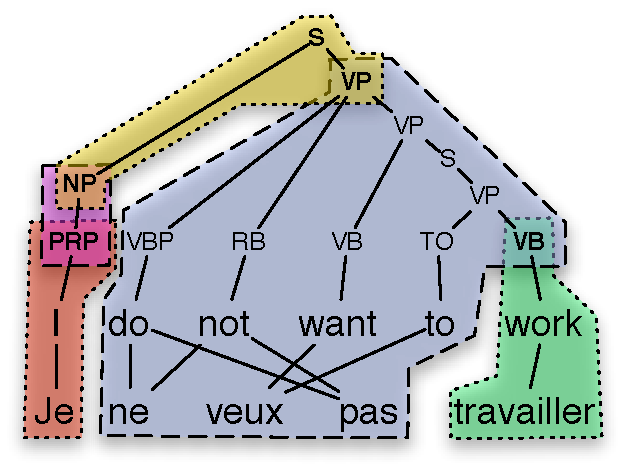
\includegraphics[scale=0.36]{JeNeVeuxPasTravailler-tsg.pdf}}
\caption{What is the best syntactic structure for SMT?}
\label{fig:models}
\end{figure}
\end{document}
